\chapter{Suchalgorithmen}
Ein Agent muss für ein bestimmtes Ziel die richtige Wahl von Aktion treffen und vorausplanen, eine Sequenz an Aktionen erstellen. Der Prozess für die Findung der Sequenz an Aktionen wird als Suche bezeichnet und durch Suchalgorithmen gefunden. Für das Finden benötigt der Agent einen Raum mit Regeln und Informationen, der im Suchproblem definiert wird.

\section{Suchproblem}
Ein Suchproblem wird definiert über einen Satz an möglichen Zuständen (\textit{states}), einen Ausgangszustand (\textit{initial state}), Zielzustände (\textit{goal states}), Aktionen (\textit{actions}), Übergangsmodel (\textit{transition model}) und Aktion-Kosten (\textit{action costs}).

Die Zustände beschreiben dabei die Umwelt und ein Ausgangszustand $s$ den Zustand des Agenten in dem der Agent startet. Ein Agent bekommt ein oder mehrere Ziele die in Zielzuständen beschrieben werden.
\begin{align*}
s = \{AtCover, GunLoaded, PlayerAlive\}
\end{align*}

Die Aktionen die ein Agent besitzt können in bestimmten Zuständen $ACTIONS(s)$ ausgeführt werden.
\begin{align*}
ACTIONS(GunLoaded) &= \{Shoot\} \\
ACTIONS(\lnot GunLoaded) &= \{Reload\}
\end{align*}

Ein Übergangsmodell $TRANSITION(s,a) = s^*$ beschreibt dabei den resultierenden Zustand $s^*$ der durch Aktionen $a$ im derzeitigen Zustand $s$ resultiert.
\begin{align*}
TRANSITIONS(GunLoaded, Shoot) &= \lnot PlayerAlive
\end{align*}

Durch eine Aktion-Kosten Funktion $ACTIONCOST(s,a,s^*)$ erhalten wir die Kosten einer Aktion $a$, welche in einem Zustand $s$ ausgeführt werden und in einen neuen Zustand $s^*$ resultieren.

%Die Lösung dabei ist die Sequenz an Aktionen die zum Zielzustand führen. Der Agent würde dieser Sequenz folgen und bei deterministischer Umwelt auch zum Zielzustand führen. Bei nichtdeterministischen Umwelten, wie Videospielen, werden so genannte closed-loop Systemen
Die Lösung für ein Suchproblem ist dabei ist die Sequenz an Aktionen, also der Plan der vom Ausgangszustand zum Zielzustand führen soll. Der gewählte Pfad sollte die geringsten Kosten von allen möglichen Lösungen haben und somit eine optimale Lösung darstellen. Der Satz an möglichen Zuständen kann dabei als Graph dargestellt werden, wobei die Kanten als Aktionen und die Knoten als Zustände dargestellt werden.

\section{Suchalgorithmen}
Das Suchproblem soll mit seinen Informationen durch einen Suchalgorithmus gelöst werden. Ein Suchalgorithmus erzeugt für seine Suche einen Suchbaum aus dem Suchproblem. Wie beim Graphen sind in Suchbäumen Knoten Zustände und Kanten Aktionen, welche zu weiteren Zuständen führen. Der Wurzelknoten ist dabei der Ausgangszustand des Agenten. Der Suchbaum beschreibt dabei Pfade zu Knoten und zum Ziel und kann mehrere Pfade zu einem gegebenen Zustand haben, aber jeder Knoten im Baum hat einen eindeutigen Pfad zurück zur Wurzel.

\begin{figure}[h]
  \centering
  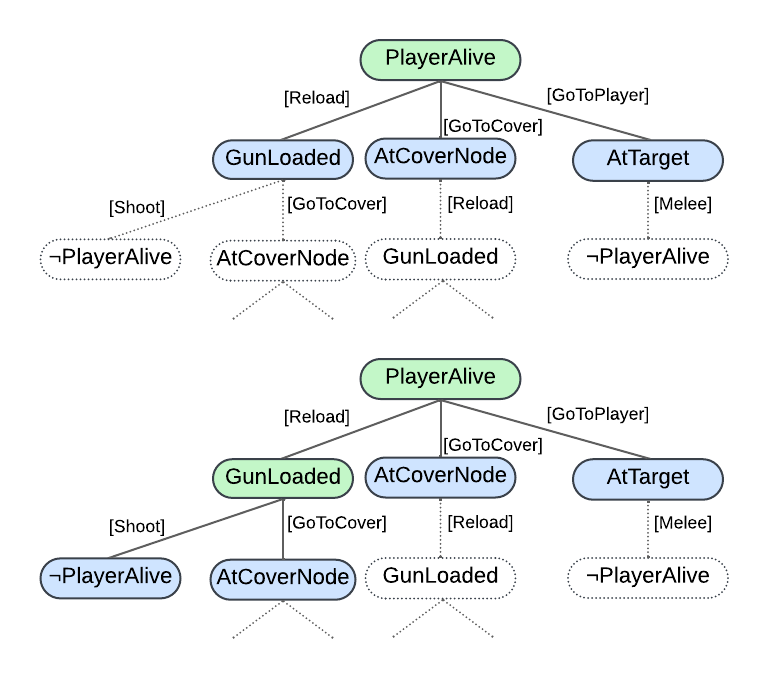
\includegraphics[width=15cm]{Suchalgorithmen/suchbaum2}
	\captionsetup{justification=justified, format=plain}
  \caption{Suchbaum: Fängt vom Ausgangszustand an und soll den Zielzustand $\lnot \textit{PlayerAlive}$ erreichen. Grüne Knoten sind expandierte Knoten, blaue Knoten sind offene gefundene Nachbarknoten und gestrichelte Knoten sind nicht entdeckte Knoten. Im Falle des Beispiels hat sich der Suchalgorithmus für den Knoten GunLoaded entschieden, da dieser optimaler als andere Nachbarknoten ist. Von dort aus ist der Zielzustand erreichbar und der Algorithmus würde eine Sequenz von Aktionen geben: \textit{[Reload,Shoot]}}
  \label{Suchalgorithmen}
\end{figure}

Bei der Expandierung schaut sich der Suchalgorithmus über die $TRANSITIONS(s)$ Funktion alle möglichen Pfade $ACTIONS(s)$ für den derzeitigen Zustand $s$ an. Zu den Pfaden werden die dazugehörigen Kind-Knoten generiert. Die Wahl zur Expansion zum nächsten Knoten variiert über den jeweiligen Suchalgorithmus und seine Bewertungsfunktion $f(n)$. Im Bereich der Suchalgorithmen wird zwischen informierten und uniformierten Algorithmen unterschieden. Informierte Algorithmen können dabei die Distanz zum Ziel über eine Heuristik schätzen, während uniformierte eine solche Schätzung nicht durchführen können. Unter die uninformierten Suchalgorithmen fallen beispielsweise die Breitensuche, Dijkstra und Tiefensuche. Zu den informierten Suchalgorithmen gehören unter anderem \textit{Greedy best-first-search} und der A* Algorithmus. Informierte Suchalgorithmen können einen Pfad durch die Informationen der Heuristik effizienter finden, als uninformierte Suchalgorithmen.

\section{A* Algorithmus}

Gehört zu den informierten und heuristischen Suchverfahren. Er ist ein so genannter vollständiger Algorithmus und findet einen Pfad zur Lösung, wenn einer vorhanden ist. Der Einsatz des Algorithmus wird oft für Routenplaner benutzt. So benutzt Godot 4.3 den A* Algorithmus für die Navigation. Der GOAP benutzt A* für das Suchen einer optimalen Sequenz an Aktionen.

\subsection{A* Bewertungsfunktion}
Suchalgorithmen, wie A* benutzen eine Bewertungsfunktion $f(n)$, welche dazu dient die Priorität eines Knoten $n$ während der Suche zu bewerten. Es werden dabei alle Kosten $g(n)$ vom Ausgangsknoten bis zu Knoten $n$ mit der Heuristik $h(n)$ des Knoten $n$ bis zum Zielknoten summiert.
\begin{align*}
f(n) = g(n) + h(n)
\end{align*}

Mit jeder Erweiterung des Pfades $n$ zu $n^{\ast}$ steigen die Kosten $g(n)$, was an den positiven tatsächlichen Aktion-Kosten $ACTIONCOST(s,a,s^*)$ der Knoten liegt. 

%g(n) + h(n) => g(n) + c(n,a,n‘) + h(n‘). 

Die Kosten-Optimalität richtet sich dabei nach einer Heuristik $h(n)$.

\subsection{A* Heuristik}
Ob A* einen optimalen Pfad findet richtet sich nach den Eigenschaften der Heuristik. Eine Heuristik hat die Eigenschaften der Zulässigkeit und Konsistenz. Ein Beispiel für eine konsistente Heuristik ist der euklidische Abstand, den man beispielsweise für die Navigation zwischen Punkten benutzten würde.

Bei einer zulässigen Heuristik werden die Kosten stets unterschätzt oder genau geschätzt. Sie bleibt im Intervall $[0, h^{\ast}(n)]$ wobei $h^{\ast}(n)$ die tatsächlichen Kosten sind.
\begin{align*}
0 \leq h(n) \leq h^*(n)
\end{align*}

Eine konsistente Heuristik muss gelichzeitig zulässig sein und die Dreiecksungleichung erfüllen. Umgekehrt muss die zulässige Heuristik nicht  Die Dreiecksungleichung stellt die Regel, dass eine Seite nicht länger sein darf als die beiden anderen Seiten zusammen.

\subsection{Beweis für Optimalität von A*}
Arbeitet der A* Algorithmus mit einer zulässigen oder konsistenten Heuristik, so wird diese den optimalen Pfad zu einem optimalen Ziel finden.

Vorraussetzung:
\begin{itemize}
\item A* expandiert auf Knoten mit der geringsten $f(n)$
\item Wir haben zwei mögliche Zielknoten:
\begin{itemize}
	\item optimaler Zielknoten $G_o$
	\item suboptimaler Zielknoten $G_s_o$
\end{itemize}
\item Eine zulässige Heuristik: $0 \leq h(n) \leq h^*(n)$
\item Einen nicht expandierten Knoten: $n$
\end{itemize}

Beweis:
\begin{enumerate}
	\item Da keine weiteren Schritte vom Zielzustand möglich sind gilt: $h(G_o) \land h(G_s_o) = 0$
	\begin{align*}
	f(G_o) &= g(G_o) + h(G_o) \\
	f(G_o) &= g(G_o) \\
	f(G_s_o) &= g(G_s_o) + h(G_s_o) \\
	f(G_s_o) &= g(G_s_o)
	\end{align*}
	Da $G_s_$ suboptimal ist folgt, dass die Pfadkosten $f(n)$ von $G_s_o > G_o$ sind und somit: $f(G_s_o) > f(G_o)$.
	\item Da $g(G_o)$ der tatsächliche Zielknoten ist und $h^*(n)$ die tatsächlichen Kosten zu $G_o$ gilt: 
	\begin{align*}
	f(n) = g(n) + h(n) &< g(n) + h^*(n) = g(G_o) \\
	f(n) &< g(G_o)
	\end{align*}
\end{enumerate}
Aus 1. und 2. folgt: $f(n) < f(G_o) < f(G_s_o)$. Somit würde A* nicht zu $G_s_o$ führen und ist mit einer zulässigen Heuristik ist optimal.


%Eine unzulässige Heuristik kann zu nicht optimalen Pfaden führen. Eine konsistente Heuristik muss zulässig sein und die Dreiecksungleichung erfüllen. So ist die Abschätzung durch Luftlinie eine konsistente Heuristik. Die Dreiecksungleichung stellt die Regel, dass eine Seite nicht länger sein darf als die beiden anderen Seiten zusammen. 
%Bezüglich Heuristik stellt sich daraus die Metrik: h(n) <= c(n,a,n‘) + h(n‘)
%c(n,a,n‘): Aktion-kosten von n bis n‘
%h(n‘): die Heuristik von n‘
%Sollte eine Heuristik konsistent sein, so sind die besuchten Zustände optimal und müssen weder in eine offene noch in eine geschlossene Liste.
%Mit einer inkonsistenten Heuristik können Pfade auftreten, welche denselben Zustand erreichen. Somit können mehrere Pfade mit unterschiedlichen Kosten aber selben Zustand in der offenen Liste auftreten, was zur höheren Zeit und Speicherkosten führt. Es gibt A* Implementationen, die dieses Problem berücksichtigen.

%\begin{align}
%Voraussetzung: f(Gs) &= g(h) + h(n); f(n) &= g(n) + h(n); h(n) \geq h*(n)$ \\
%Behauptung: $f(Gs) > f(n)$
%\end{align}
